
%---------------------------------------%
\section{Question 5 (Sample Variant 2)[25 marks]}

\begin{itemize}
%----------------------------------------------------- %
\item[(a)] \textbf{\textit{Binary Channels (5 Marks)}}\\

Consider the binary channel in the figure below.
\begin{figure}[h!]
\centering
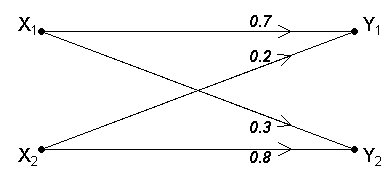
\includegraphics[width=0.7\linewidth]{./10Bnet3}
\caption{}
\label{fig:10Bnet3}
\end{figure}

\begin{itemize}
\item[(i)] (1 Marks) Determine the channel matrix of the channel
\item[(ii)] (2 Marks)  Find P($Y_1$) and P($Y_2$) when P($X_1$) = 0.7 and P($X_2$) = 0.3.
\item[(iii)] (2 Marks)  Find the joint probabilities P($X_1$, $Y_1$) and P($X_2$,$Y_2$).
\end{itemize}